\documentclass[10pt]{report}
\usepackage[utf8]{inputenc}
\usepackage{float}
\usepackage{amsmath}
\usepackage{systeme}
\usepackage{bbold}
\usepackage{graphicx}
\usepackage{float}
\usepackage{caption}
\usepackage{subcaption}
\usepackage{fancyhdr}
\usepackage{tcolorbox}
\usepackage{mathrsfs}
\usepackage{fancybox}
\usepackage{calc}
\usepackage{setspace}               % for LINE SPACING
\usepackage{physics}
\usepackage{braket}
\usepackage{hyperref}
\numberwithin{equation}{section}

%\definecolor{main}{HTML}{5989cf}    % setting main color to be used
%\definecolor{sub}{HTML}{cde4ff}     % setting sub color to be used

%\tcbset{
%    sharp corners,
%    colback = white,
%    before skip = 0.2cm,    % add extra space before the box
%    after skip = 0.5cm      % add extra space after the box
%}                           % setting global options for tcolorbox

\newtcolorbox{boxA}{
    sharpish corners, % better drop shadow
    boxrule = 0pt,
    toprule = 4.5pt, % top rule weight
    %%enhanced,
    %%fuzzy shadow = {0pt}{-2pt}{-0.5pt}{0.5pt}{black!35} % {xshift}{yshift}{offset}{step}{options} 
}



\usepackage[T1]{fontenc}
\usepackage{geometry}
\geometry{verbose,tmargin=3cm,bmargin=3cm,lmargin=3cm,rmargin=3cm}
%\geometry{hmargin=2.5cm,vmargin=2.5cm}
\usepackage{units}
\usepackage{textcomp}
\usepackage{amstext}
\usepackage[numbers]{natbib}

%\makeatletter

%%%%%%%%%%%%%%%%%%%%%%%%%%%%%% LyX specific LaTeX commands.
\newcommand{\noun}[1]{\textsc{#1}}
%% Because html converters don't know tabularnewline
\providecommand{\tabularnewline}{\\}

%%%%%%%%%%%%%%%%%%%%%%%%%%%%%% User specified LaTeX commands.
\usepackage{fancyhdr}
\setlength{\headheight}{14.49998pt}
%\addtolength{\topmargin}{-2.49998pt}
\pagestyle{fancy}
\fancyhf{}
\rhead{Flaurent \textsc{HEULLY--ALARY -- Thesis Report}}
\lhead{\textsc{University Paul Sabatier}}
\cfoot{\thepage}

\makeatother

\usepackage{babel}
\makeatletter
\addto\extrasfrench{%
   \providecommand{\og}{\leavevmode\flqq~}%
   \providecommand{\fg}{\ifdim\lastskip>\z@\unskip\fi~\frqq}%
}

%\makeatother
\begin{document}
%\begin{center}
%\noun{\large{}University Paul Sabatier 2021}{\large\par}
%\par\end{center}

%\begin{center}
%\par\end{center}
\begin{titlepage}
\newcommand{\HRule}{\rule{\linewidth}{0.5mm}}
\center
\textsc{\LARGE
University \noun{Paul Sabatier}
} \\[1cm]
%\includegraphics[scale=0.5]{LOGO.jpg} \\[1cm]
\HRule\\[0.4cm]
{ \huge \bfseries Un joli titre \\[0.15cm] }
\HRule\\[1.5cm]
Flaurent HEULLY--ALARY
\\[1cm]
\today \\ [1cm]
\end{titlepage}
\begin{center}
\thispagestyle{plain}
\par\end{center}
\large
\tableofcontents
\newpage
\section{Introduction}
For a long time theory has tried to match experiments, reproducing their results and trying to understand the mechanism at the origin of the different properties studied.
%Mini intro

\chapter{Theory and Methodology}

\section{Model Hamiltonian}

\subsection{Spin Hamiltonian}

\subsection*{Heiseinberg Hamiltonian}
The most well-know Spin Hamiltonian used to describe the magnetic interaction between a pair of spin located on different magnetic centres is the Heiseinberg-Dirac-Van Vleck (HDVV) Hamiltonina, written as:
\begin{equation}\label{Hheis}
    \hat{H}_{HDVV}=-\sum_{i,j} J_{ij} \hat{\vb S}_i \cdot \hat{\vb S}_j
\end{equation}

where $J_{i,j}$ is the coupling constant, $\hat{\vb S_i}$ and $\hat{\vb S_j}$ are the spin operators working on site $i$ and $j$.
Several conventions exist for this Hamiltonian, with negative sign and/or a factor of 2 in front.  
The coupling constant $J$ can be either positive or negative depending on the magnetic properties of the system, a positive value indicate ferromagnetism with magnetic moment aligned while negative indicate antiferromagnetism with opposite alignement of magnetic moments.
This Hamiltonian is regarded as a Spin Hamiltonian as it only invoke the spin degree of freedom of the system and is still to this day used in the description of the isotropic coupling in magnetic systems.

The $J$ constant is defined as an effective integral as it involves several mechanisms:
\begin{itemize}
    \item[1-] Direct exchange originating from the exchange integral $K$.
    \item[2-] Indirect exchange involving ionic determinants.
    \item[3-] Super-exchange where a diamagnetic bridging ligand open new pathway for exchange mechanisms.
\end{itemize}

The origins and contributions of these mechanisms to the effective integral can be understood from the Hubbard Hamiltonian in the case of two electrons in two orbitals.
Up to the second order perturbation theory, the following expression can be obtained for the effective integral $J$:
\begin{equation}
    J=2K-\frac{4t^2}{U}
\end{equation}
Where $K$ is the exchange integral which is always positive, $t$ the hopping integral between the two orbitals and $U$ the on site Coulomb repulsion.
This expression shows the competition between a ferromagnetic component ( direct exchange $K$>0) and an antiferromagnetic one (indirect exchange).
The contribution of super-exchange cannot be estimated at second-order and requires going up to fourth-order pertubation giving a similar expression:
\begin{equation}
    J=2K-\frac{4t_{eff}^2}{U}
\end{equation}
Where $t_{eff}$ is now an effective hopping integral involving the bridging ligand, the hopping term between metallic to ligand being much larger than the metallic to metallic one, the $t$ term is usually neglected in this expression.
Note that the perturbation expansion is valid only in case of $U>>t$, when the system's behavior is not dominated by delocalisation that would render the HDVV Hamiltonian inadecate.

\subsection*{Ising Hamiltonian}

The eigenfunctions of the Heiseinberg Hamiltonian are eigenfunctions of the $\hat{\vb S}^2$ operator, making them mostly multi-determinental functions which can only be obtained via specific computation method.
To draw an easier picture, it is possible to restrict the spin vector to its component along the $z$ axis alone.
\begin{equation}
    H_{ising}=- \sum_{i,j} J_{ij} \hat{\vb S}_{z,i} \hat{\vb S}_{z,j}
\end{equation}
The magnetic moment of each lattice site are now considered to align themselves with the $z$ axis at all time, taking a $\pm 1$ value.
The main advantage of this approximation is that the eigenfunctions of this Hamiltonian are now mono-determinantal functions opening up the extraction to new computation methods. 
It also reduces the analytical derivation allowing to work on larger systems without the need to diagonaize large matrices.

\subsection{Mononuclear Anisotropy}

\par Effects such as Spin-Orbit-Coupling (SOC) tend to create anisotropy in the system that cannot be described only by eq(\ref{Hheis}). 
More specifically on mononuclear systems (only one magnetic centre) with a ground state of spin larger or equal to one, a lift of degeneracy between the different $M_S$ component of a same $S$ state can be observed even in the absence of magnetic field, this phenomenon is called Zero-Field-Splitting.
%In reality it is not correct to address these states as spin states of spin $S$ with an $M_S$ component, they should be considered as spin-orbit states created from the mixing of multiple spin states that cannot be described by an $S$ and $M_S$ value but pseudo-spin.
%However, in transition metals complexes the relativistic effects remain "small" and the spin becomes a "not-too-bad" quantum number. 
%The low-lying SO-states are then mainly composed of combination of $\pm M_S$ components of a single spin states $S$, it then becomes "acceptable" to name them from the spin state it is composed.
The associated Spin Hamiltonian is written:
\begin{equation}\label{SDS}
    \hat{H}_{ZFS}=\hat{\vb S} \cdot \overline{\overline{D}} \cdot \hat{\vb S}
\end{equation}
Where $\hat{\vb S}$ is the spin vector of the ground state and $\overline{\overline{D}}$ is a two rank symmetric tensor, in an arbitrary frame it is composed of six different parameters.
\begin{equation}
    \overline{\overline{D}}=\begin{pmatrix}
        D_{xx} & D_{xy} & D_{xz}\\
        D_{xy} & D_{yy} & D_{yz}\\
        D_{xz} & D_{yz} & D_{zz}
    \end{pmatrix}
\end{equation}
This tensor can be reduced to three parameters by diagonalization, $\textit{i.e}$ expressing them in the the tensor principal axes that define the magnetic anisotropy axes.
Going further as to work with traceless tensor allow us to use only two parameters, by convention the z-axis is taken as the main magnetic axis with D the axial parameter:
\begin{equation}\label{ParametreD}
    D=D_{zz}-\frac{1}{2}(D_{xx}+D_{yy})=\frac{3}{2}D_{zz}
\end{equation}
and the rhombic term:
\begin{equation}\label{ParametreE}
    E=\frac{1}{2}(D_{xx}-D_{yy})
\end{equation}
With $|D| \geq 3E \geq 0$. 
The ZFS Hamiltonian can then be written:
\begin{equation}  %Différentes conventions??%
    \hat{H}_{ZFS}=D (\hat{S}_z^2-\frac{1}{3}\hat{S}^2)+E(\hat{S}_x^2-\hat{S}_y^2)
\end{equation}
A positive value of D indicates that the ground state is mainly composed of the $M_S$=0 component meaning that the projection of the spin moment along the $z$-axis is close to zero resulting in a easy-plane magnetism. 
On the contrary if D<0, the ground state is formed from the $M_S$=$\pm M_{Smax}$ components with a maximum projection of spin moment along the $z$-axis resulting in an easy-axis magnetism.
For a ground state with spin larger than one and a half, other terms may appear but will not be reported in this work. %(alors peut-être)

In the case of a triplet S=1 ground stat such as a nickel Ni (II) complex, the matrix representation of hamiltonian (\ref{SDS}) in a random set of axis:
\begin{center}
\begin{tabular}{ c | c c c}
    $H_{ZFS}$ & $\ket{1,-1}$ & $\ket{1,0} $& $\ket{1,1}$ \\
    \hline
    $\bra{1,-1} $&  $\frac{1}{2}(D_{xx}-D_{yy})+D_{zz}$ & $-\frac{\sqrt{2}}{2}(D_{xz+iD_{yz}}) $ & $\frac{1}{2}(D_{xx}-D_{yy}+2iD_{xy})$ \\
    $\bra{1,0}$ & $-\frac{\sqrt{2}}{2}(D_{xz-iD_{yz}})  $& $ D_{xx}+D_{yy}  $&$ \frac{\sqrt{2}}{2}(D_{xz}+iD_{yz})$ \\
    $\bra{1,1} $& $ \frac{1}{2}(D_{xx}-D_{yy}-2iD_{xy}) $& $\frac{\sqrt{2}}{2}(D_{xz}-iD_{yz})$  & $\frac{1}{2}(D_{xx}+D_{yy})+D_{zz} $ \\
\end{tabular}\\
\end{center}
In the magnetic frame, this matrix becomes:
\begin{center}
\begin{tabular}{c | c c c}
    $H_{ZFS}$ & $\ket{1,-1}$ & $\ket{1,0} $& $\ket{1,1}$ \\
    \hline
    $\bra{1,-1}$ & $\frac{1}{2}(D_{XX}+D_{YY})+D_{ZZ}$ & 0 & $\frac{1}{2}(D_{XX}-D_{YY})$\\
    $\bra{1,0}$ & 0 & $D_{XX}+D_{YY}$ & 0\\
    $\bra{1,1}$ &  $\frac{1}{2}(D_{XX}-D_{YY})$ & 0 & $\frac{1}{2}(D_{XX}+D_{YY})+D_{ZZ}$
\end{tabular}
\end{center}
Removing the trace from the tensor and applying the convention from eq(\ref{ParametreD}) and eq(\ref{ParametreE}) we get:
\begin{center}
\begin{tabular}{c | c c c}
    $H_{ZFS}$ & $\ket{1,-1}$ & $\ket{1,0}$ & $\ket{1,1}$\\
    \hline
    $\bra{1,-1}$ & $\frac{1}{3}D$ & 0 & E\\
    $\bra{1,0}$ & 0 & $\frac{2}{3}D $& 0\\
    $\bra{1,1}$ & E & 0 & $\frac{1}{3}D$
\end{tabular}
\end{center}
Note that in the case of an even number of unpaired electron, the D and E parameter can be estimated directly from the energy spectrum.
\begin{figure}
    \centering
    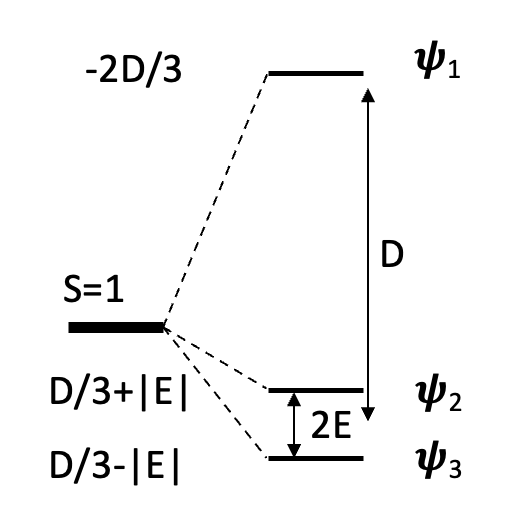
\includegraphics[width=0.4\textwidth]{Images/SpectreZFS.png}
    \caption{Schematic representation of the three lowest SO-state undergoing ZFS in the case of triplet ground state.}
    \label{SpectreZFS}
\end{figure}
In the case of a triplet ground state, diagonalizing the model Hamiltonian matrix gives the three eigenvalues:
\begin{align}
    E_1&=-\frac{2}{3}D\\
    E_2&=\frac{1}{3}D+E\\
    E_3&=\frac{1}{3}D-E
\end{align}
with the eigenvectors:
\begin{align}
    \psi_1&=\ket{1,0}\\
    \psi_2&=\frac{1}{\sqrt{2}}(\ket{1,-1}+\ket{1,1})\\
    \psi_3&=\frac{1}{\sqrt{2}}(\ket{1,-1}-\ket{1,1})
\end{align}
leading to the extraction of the D and E terms from the energy values:

\begin{equation}
    D=\frac{1}{2}(E_2+E_3)-E_1
\end{equation}
and
\begin{equation}
    E=\frac{1}{2}(E_2-E_3)
\end{equation}



\subsection{Polynuclear Anisotropy}
Opening the study to multiple magnetic center introduces weak couplings between the magnetic moments of each center. 
This coupling between two sites A and B with a least of magnetic elctron each, is called exchange interaction and is described by the following Giant Spin Hamiltonian.
\begin{equation}
    \hat{H}_{AB}=\hat{\vb S}_A\cdot \overline{\overline{D}} \cdot \hat{\vb S}_B
\end{equation}
The spin-spin interaction tensor $\overline{\overline{D}}$ describes Zero-Field-Splitting the same way as before but now between two sites $A$ and $B$, two parameters $D$ and $E$ can be defined similarly. 
This Hamiltonian is suitable for system with a ground state of spin larger or equal to one.
It is also possible to study cases where mixing with low-lying excited states occurs by decomposing the tensor $\overline{\overline{D}}$ in three terms.

\begin{equation}
    \hat{H}_{AB}=J(\hat{\vb S}_A \cdot \hat{\vb S}_B) + \hat{\vb S}_A \cdot\overline{\overline{D}}_{AB} \cdot \hat{\vb S}_B + \vb{d}_{AB} \cdot (\hat{\vb S}_A \cross \hat{\vb S}_B)
\end{equation}

Where the first term is the isotropic exchange, extending this coupling to more than two center this term becomes equivalent to the HDVV Hamiltonian from (\ref{Hheis}).
The two following terms describe the anisotropic exchange with the symmetric tensor of exchange $\overline{\overline{D}}_{AB}$ and the antisymmetric exchange $\vb{d}_{AB}$ also called Dzyaloshinskii-Moriya pseudo-vector interaction.
For couplings involving more than one unpaired electron per site, local tensor are introduced:
\begin{equation}
    \hat{H}_{AB}=J(\hat{\vb S}_A \cdot \hat{\vb S}_B) + \hat{\vb S}_A \cdot\overline{\overline{D}}_{AB} \cdot \hat{\vb S}_B + \vb{d}_{AB} \cdot (\hat{\vb S}_A \cross \hat{\vb S}_B) +\hat{\vb S}_A \cdot\overline{\overline{D}}_{A} \cdot \hat{\vb S}_A +\hat{\vb S}_B \cdot\overline{\overline{D}}_{B} \cdot \hat{\vb S}_B
\end{equation}

The matrix representation of two spin 1/2 systems interacting is the following:
\begin{center}
    \begin{tabular}{c | c c c c}
        $H_{MS}$ & $\ket{1,-1}$ & $\ket{1,0}$ & $\ket{1,1}$ & $\ket{0,0}$\\
        \hline
        $\bra{1,-1}$ & $\frac{J}{4}+\frac{D_{zz}}{4}$ & $\frac{D_{xz}-iD_{yz}}{2\sqrt{2}}$ & $\frac{(D_{xx}-D_{zz}-2iD_{xy})}{4} $& $\frac{d_y+id_x}{2\sqrt{2}}$\\
        $\bra{1,0}$ & $\frac{D_{xz}+iD_{yz}}{2\sqrt{2}}$ &$ \frac{J}{4} -\frac{D_{zz}}{4} +\frac{(D_{xx}+D_{yy})}{4}$& $-\frac{D_{xz}-iD_{yz}}{2\sqrt{2}}$ & -$\frac{id_z}{2}$ \\
        $\bra{1,1}$ &$\frac{(D_{xx}-D_{zz}+2iD_{xy})}{4} $ & $-\frac{D_{xz}+iD_{yz}}{2\sqrt{2}}$ & $\frac{J}{4}+\frac{D_{zz}}{4}$ & $\frac{d_y-id_x}{2\sqrt{2}}$\\
        $\bra{0,0}$ & $\frac{d_y-id_x}{2\sqrt{2}}$  & $\frac{id_z}{2}$  &$\frac{d_y+id_x}{2\sqrt{2}}$  & $-\frac{3J}{4}-\frac{D_{zz}}{4}-\frac{(D_{xx}+D_{yy})}{4}$\\
    \end{tabular}
\end{center}
From this matrix we notice that the Dzyaloshinskii-Moriya interaction create a coupling between the singlet with the three $M_S$ components of the triplet state.
As for the symmetric tensor of anisotropic exchange, it only couples the three component of the triplet which undergo a splitting in energy.
At the isotropic level, the difference between the triplet and singlet state is given by $\Delta E=J$, but with the inclusion of the anisotropic terms this becomes much more complex. 
As opposed to the Zero-Field Splitting mechanism, it is impossible to obtain values for these interactions from the energy spectrum only, as such they will be extraced from effective Hamiltonian theory.
Note that now the application of this Hamiltonian is not restricted to a ground state with $S\ge1$ but can be used for a singlet or doublet case.
All of these considerations are only possible in the strong exchange limit where the isotropic coupling is strong compared to the anisotropic interactions.

%So far, we have assumed the colinearity of spin moments, the introduction of the antisymmetric exchange now favor a \textit{spin canting} where the spin moment are no longer parallel or antiparallel resulting in weak ferromagnetism in otherwise antiferromagnetic systems.

\section{Methodology}

All types of calculations discussed here after have for purpose to solve, in some way, the Schrodinger Equation:

\begin{equation}
    \hat{H}\Psi_i=E_i\Psi_i
\end{equation}
Where $\hat{H}$ is an Hamiltonian used to describe the system studied, $E_i$ is the energy associated to the wave-function $\Psi_i$. 
The solutions $E_i$ of this problem are obtained pretty straightforwardly by diagonalizing the Hamiltonian except that in most cases, the $\Psi_i$ vector are not known beforehand.
The Hamiltonian discussed before is called exact electronic Hamiltonian as it encapsulate all the electronic and nuclear interaction of the system, it is written as follow in atomic units:

\begin{equation}
    \hat{H}=-\sum_{i=1}^{N}\nabla_i^2-\sum_{A=1}^{M}\frac{1}{2M_A}\nabla_A^2%
    -\sum_{i=1}^{N}\sum_{A=1}^{M}\frac{Z_A}{|r_i-R_A|}+\sum_{i=1}^{N}\sum_{j<i}^{N}\frac{1}{r_{ij}}%
    +\sum_{A=1}^{M}\sum_{B>A}^{M}\frac{Z_A Z_B}{|R_A-R_B|}
\end{equation}
Where $r_i$ is the position vector of the $i$th electron, $R_A$ the position vector of the $A$th nucleus with atomic number $Z_A$ and mass $M_A$.
This Hamiltonian can be simplified in the context of the Born-Oppenheimer approximation, the electrons are considred to adapt instantly to the movement of the nuclei, the latter's position can be fixed and taken out of the Hamiltonian.
This approximation is justified with the fact that the electrons are much lighter than the nuclei. 

\begin{equation}\label{Helec}
    \hat{H}_{elec}=-\frac{1}{2}\sum_{i=1}^{N}\nabla_i^2%
    -\sum_{i=1}^{N}\sum_{A=1}^{M}\frac{Z_A}{|r_i-R_A|}+\sum_{i=1}^{N}\sum_{j<i}^{N}\frac{1}{|r_i-r_j|}%
\end{equation}

This Hamiltonian describes the electronic problem while the nuclei contribution is set aside in a constant, having for only effect a shift in the overall energy spectrum. 
While this greatly simplify the equations, it is still not solvable analyticaly and several approximations were developped to tackle this problem. %
One common point to all the methods that were used in this work rely on the construction of molecular orbitals (\textbf{MO}) as expansions of atomic orbitals (\textbf{AO}).

\begin{equation}
    \psi_k=\sum_{i}c_i \phi_i
\end{equation}

Where $\psi_k$ is the $k$th MO built from the AO $\phi_i$ with the coefficient $c_i$. 
This expansion rely on a supposedly infinite number of AO but in real case application this is not achievable and will thus be restricted to a finite number of basis functions.
As the eletronic Hamiltonian does not include any information about spin, it will be included within a so called spin orbital with the introduction of two orthonormal function $\alpha(\omega)$ and $\beta(\omega)$, \textit{i.e} spin up or down function, with $\omega$ an unspecified spin variable.
From each spatial molecular orbital, two spin orbital can be created such that:
\begin{equation}
    \chi_i=\begin{cases}
    \psi_i(r)\alpha(\omega)\\
    \quad or \\
    \psi_i(r)\beta(\omega)
    \end{cases}
\end{equation}
This definition for the spin orbital is well adapted for closed shell systems where all molecular orbitals are doubly occupied, the spatial part for any spin orbital is the same for both spin function defining the restricted formalism.
Such definition changes when working with open shell system, \textit{i.e} some orbitals are singly occupied  necessiting the application of unrestricted formalism.

\subsection{Hartree-Fock Method}
The cornersone of $ab$ $initio$ calculation in quantum chemistry is the Hartree-Fock method which is usually the initial step for computing a first approximation of the wave function in molecules. 
It is a variational approach that aims to treat the N-electron problems as problem of N non interacting electrons in the presence of an average potential replicating interactions between them, it is in this sense a mean-filed theory.
This wave-function is constructed on the optimisation of a single Slater determinant $\Psi$:
\begin{equation}
    \Psi(x_1,x_2,\ldots,x_N)=\frac{1}{\sqrt{N!}}
    \begin{vmatrix}
        \chi_i (x_1) & \chi_j (x_1) & \cdots & \chi_k (x_1)\\
        \chi_i (x_2) & \chi_j (x_2) & \cdots & \chi_k (x_2)\\
        \vdots & \vdots &   &  \vdots\\
        \chi_i (x_N) & \chi_j (x_N) & \cdots & \chi_k (x_N)\\
    \end{vmatrix}
\end{equation}
Where $\chi_i$ are spin orbitals and the variable $x_i=\{r_i,\omega_i\}$, it involves all combination of all $N$ electrons in all $k$ spin orbitals. 
We introduce the shorthand notation for such determinant $\Psi(x_1,x_2,\ldots,x_N)=\ket{\chi_1\chi_2\ldots\chi_k}$ showing only the diagonal elements of the determinant.

The way to obtain the best adapted Hartree-Fock wave function comes through the resolution of the Roothan's equation:
\begin{equation}\label{Roothans}
    FC=SC\epsilon
\end{equation}
$S$ is the overlap matrix of the basis function, $\epsilon$ the matrix of orbital energies and C is the matrix of the trial vector.
The Fock operator $F$ is defined as:
\begin{equation}
    \hat{F}(i)=\hat{h}(i)+\sum_{j}^{N/2}[2\hat{J}_{j}(i)-\hat{K}_{j}(i)]
\end{equation}

The core-Hamiltonian $\hat{h}(i)$ is a mono-electronic operator that contains the kinetic energy operator of the $i$th and coulomb repulsion with the fixed nuclei. 
The two bieletronic operator $\hat{J}_{j}(i)$ and $\hat{K}_{j}(i)$ describe the coulomb repulsion and exchange mechanism between the i$th$ electron and the rest.
These operator carry a direct dependance on the trial vectors from eq \ref{Roothans} as such, the Roothan's equation are non-linear and will be solved iteratively following a $Self$ $Consistent$ $Field$ (SCF) procedure.


\subsection{Complete Active Space Self Consistent Field}

For most of magnetic systems, a single reference wave function is not enough as the system is usually not closed-shell and present one or more unpaired electron. Hence, its ground state is described by a wave function composed of several determinants.
One of the most used method to introduce multiple reference in the wave function is called $Complete$ $Active$ $Space$ $Self$ $Consistent$ $Field$ ($CASSCF$). 
Compared to the Hartree-Fock theory where two types of orbitals (occupied and unoccupied) were considered, in CASSCF theory orbitals are separeted in three sub-space. The inactive orbitals are doubly occupied throughout the calculation, virtual orbitals will stay empty while the active orbitals have a variable occupancy ranging from zero to two electrons.
These active orbitals define the active space into which a configuration interaction will be realised computing all the determinants possible within this sub-space. 
\begin{figure}
    \centering
    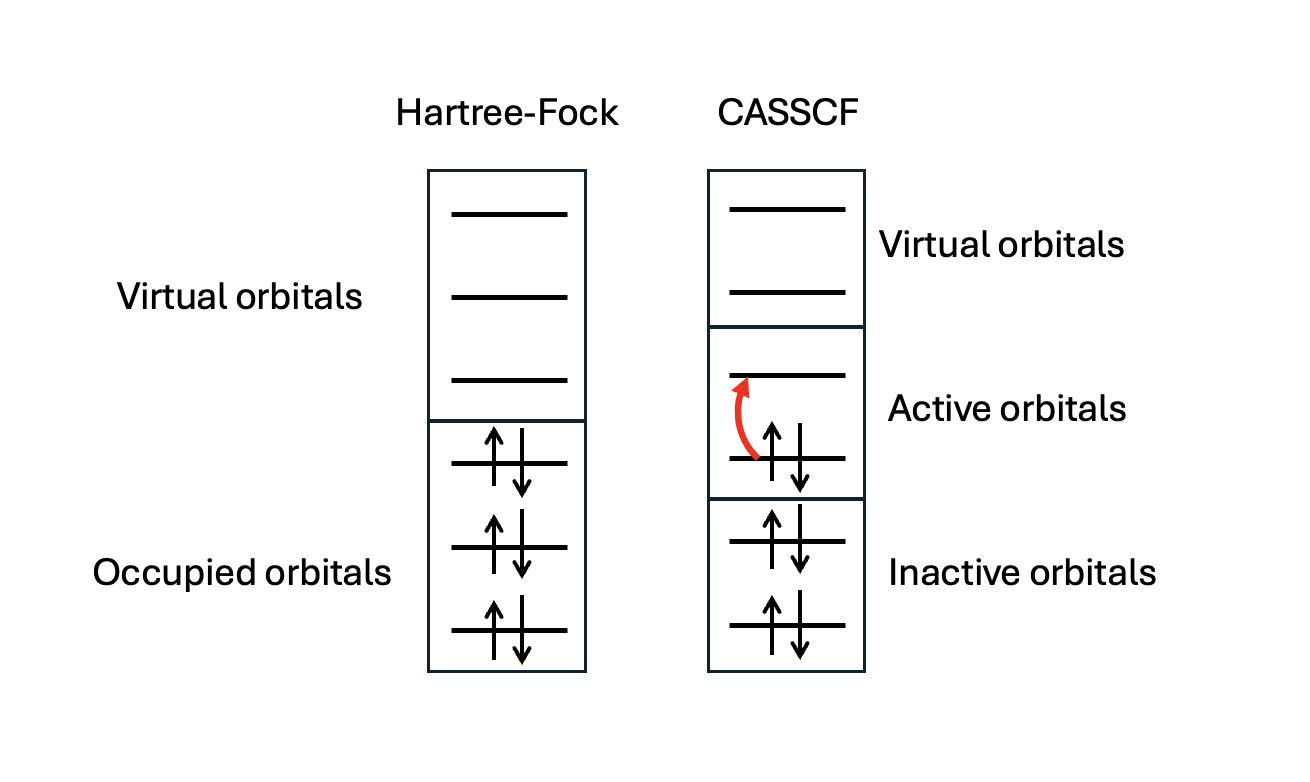
\includegraphics[width=0.8\textwidth]{Images/EspaceCAS.png}
    \caption{Difference between the orbitals space in Hartree-Fock and CASSCF Theory}
    \label{CAS}
\end{figure}
As the number of determinant grows significally with the number of orbitals included in the active space, this method is quite costly and its size becomes a limiting factor for the calculations.
The new wave functions is now written as an expansion of Slater determinant which is obtained via a SCF procedure where both the expansion coefficients and orbitals are optimised as to minimize the Schrodinger Equation. 
This double optimisation scheme can render the convergence troublesome, as such the definition of the active space and the choice of the starting orbitals becomes crucial. One usually starts from a set of orbitals previously obtained via an Hartree-Fock calculation.
For computation of magnetic properties in metallic systems, the minimum active space should consists of the magnetic orbitals, $i.e$ the singly occupied d-orbitals of the metalic centers, this can later be extended to all of the 3-d orbitals of the metal as well as some orbitals of the ligands.
As a result of the CASSCF method we obtain the energies of all states included in the calculation and a new set of orbitals into which they are expressed. 
This calculation takes into account the correlation between the electrons inside the active space in the mean field created by the other electrons. 
While this method provides the non-dynamical correlation, it fails to capture the correlation with the inactive electron and their reponse to excitations, called dynamic-correlation and the need to look further appears.


\subsection{Perturbation Theory}

Perturbative treatment can be applied to extract the dynamical correlation of the mono and diexcitations that is left out from simple CASSCF calculation. For such calculation, one can use the CASPT (Complete Active Space Perturbation theory)
or the NEVPT (N-electron valence state perturbation theory). Both of these methods rely on the assumption that the Hamiltonian can be partitioned into a zeroth order term and a perturbation with the parameter $\lambda$:

\begin{equation}
    \hat{H}=\hat{H}^{(0)}+\lambda\hat{H}^{(1)}+\lambda^2 \hat{H}^{(2)}+\ldots
\end{equation}


The wave function and energy are expanded in a similar way and the zeroth order term $\Psi_{(0)}^{0}$ is chosen to be the CASSCF wave function. 
The effect of the configurations outside of the active space on the energy and the wave function is estimated though perturbation theory and the expansions of the equations allows one to obtain the corrected energies
usually at second order of perturbation with CASPT2 or NEVPT2. These two method mainly differs from their chose of zeroth-order Hamiltonian, CASPT2 rely on a monoelectronic Hamiltonian built from a one electron Fock operator that falls back to the Moller-Plesset Hamiltonian in single reference case. 
This treatment may lead to what is called "intruder states" where low-lying states induce divergence in the denominator of the correction term where a difference of energy is taken. Several approach have been adapted such a the introduction of a $level$ $shift$, real or imaginary, as to fix this divergence.
In case of NEVPT2, the zeroth-order Hamiltonian is a bi-electronic Dyall Hamiltoninan which in itself include a shift in energy between state from inside or outside the active space preventing the appearance of intruder states.
One should add that this correlation is considered contracted as these methods do not act upon the coefficients inside the wave functions but only on the energies.

\subsection{Difference dedicated configurational interaction}

To get a full picture of the dynamic correlation one has to go to Multi-Referential-Configuration-Interaction (MRCI) methods.
This method allows to introduce new determinants in the wave-function that do not belong to the CASSCF space, this way not only the energies but the wavefunction itself is revised.
While very promising this method is not applicable to any real systems because of the number of determinants to include in the CI expansion, the cost of calculation becoming too high one has to truncate the MRCI space.
Restricting the CI to all the simple and double excitations is still not feasible as they are too numerous, but some of them can be left out of the calculations. 
These excitations are classified into eight categories depending on the number of hole/particle created represented on figure \ref{DDCI}. 
A hole is an excitation from a inactive orbital to an active or virtual orbital, while a particle is an excitation from an active or inactive orbital to a virtual one.

\begin{figure}
    \centering
    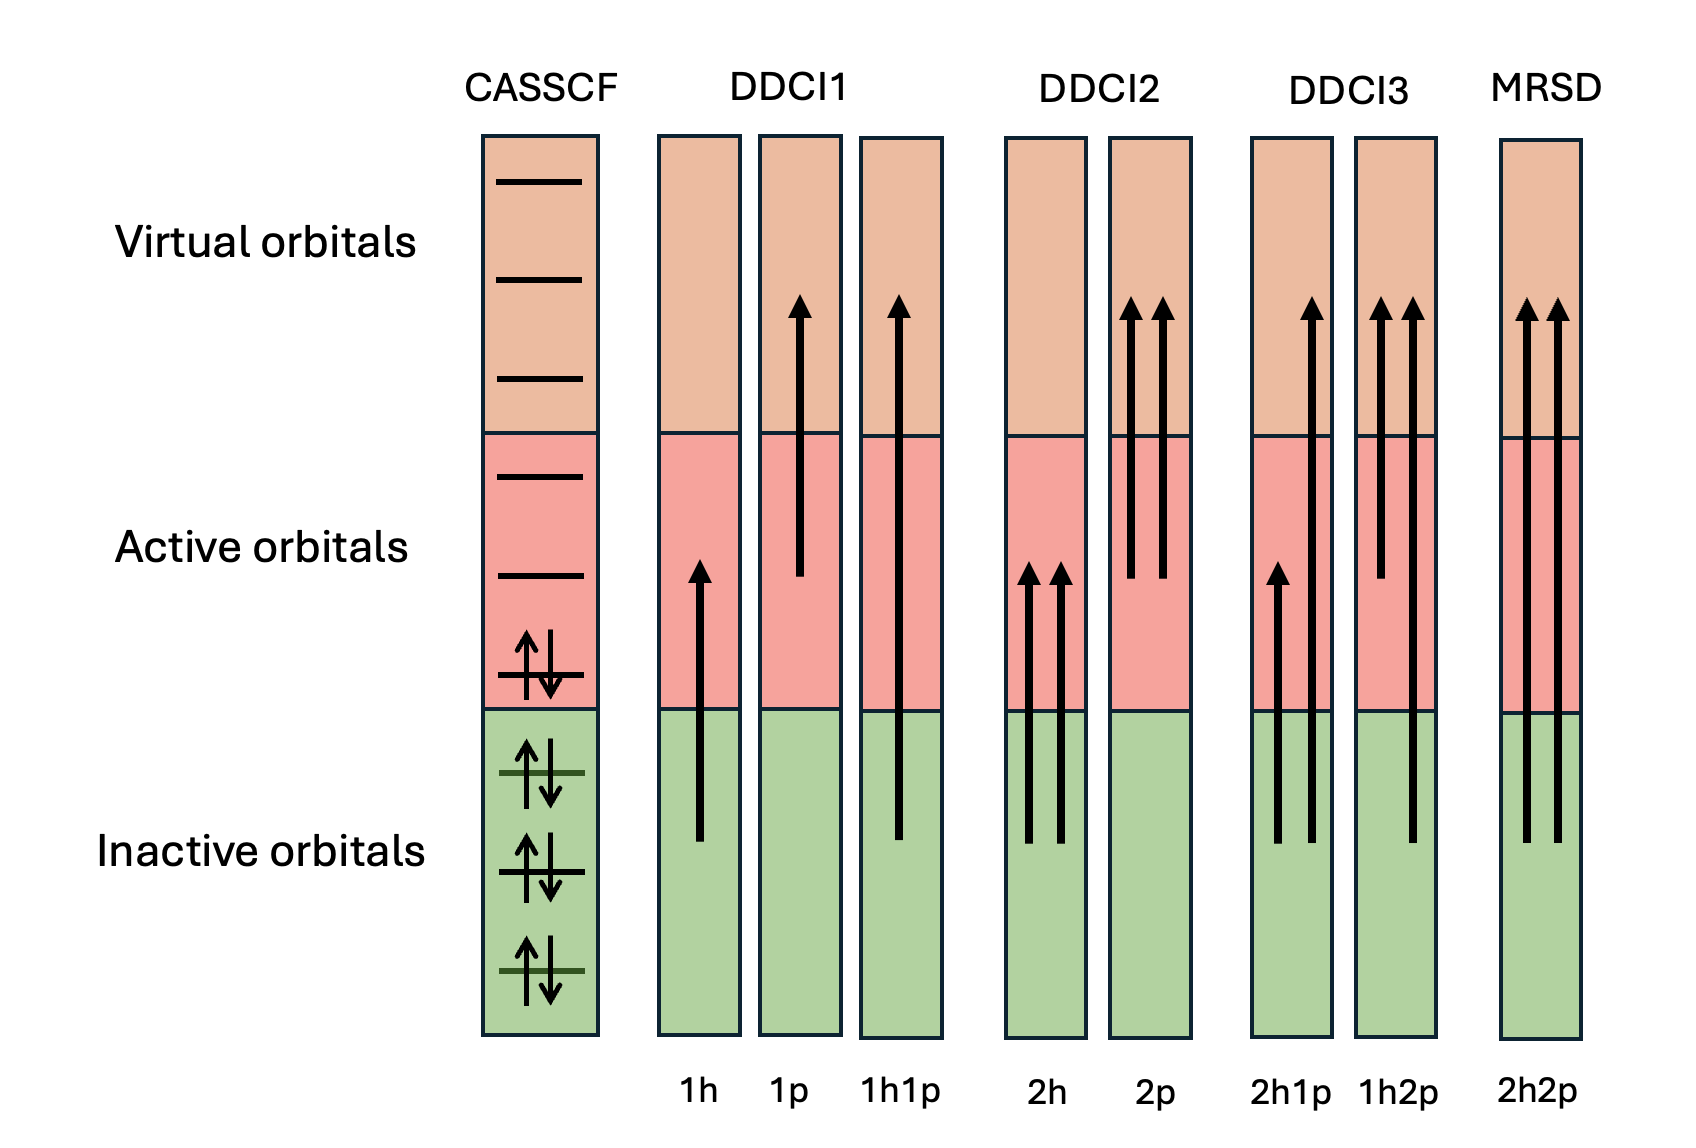
\includegraphics[width=0.8\textwidth]{Images/DDCI.png}
    \caption{Classes of excitations and associated DDCI method}
    \label{DDCI}
\end{figure}
The most troublesome excitations are the one generating two holes and two particles (2h-2p) as they are the most numerous, but it can be shown at second order of perturbation that they do not contribute to the energy difference but only act as a shift of the diagonal energies.
As such they can be neglected giving rise to a variant of MRCI called Difference-Dedicated-Configurational-Interaction (DDCI). 
Three sub-variant of DDCI exists taking into account differents classes of excitations as pictured on fig \ref{DDCI}
It has been established that the extraction of magnetic coupling involving bridging ligand requires the use of the DDCI3 method to provide good estimates.

\subsection{Density functional theory}

Another way to get a description of the electronic structure of is through density functional theory (DFT).
The main interest of such method is the description of the ground state properties through the determination of the ground state energy $E_0$ following the variationl theorem
\begin{equation}
    E_0 = \min \bra{\Psi} \hat{H} \ket{\Psi}
\end{equation}
Here, the eletronic wavefunction of the molcule $\Psi$ is approximated to a single Slater determinant obtained from the determination of the electronic density $\rho(\vb r)$:
\begin{equation}
    \rho(\vb r)=N\int |\Psi(\vb x_1 \ldots \vb x_N)|^2 ds_1 dx_2 \ldots dx_N
\end{equation}
The Hamiltonian\ref{Helec} can be written:
\begin{equation}\label{Hop}
    \hat{H}=\hat{T} + \hat{V}_{ee} + \hat{V}_{ne}
\end{equation} 
with $\hat{T}$ the kinetic energy operator, $\hat{V}_{ee}$ the electron-electron interaction operator and $\hat{V}_{ne}$ the nuclei-electron interaction operator. 
Solving the Shrod

by replacing $v_{ne}(\rho\vb r)$ by a known external potential $v(\vb r)$, one can obtain the ground state wave function $\Psi$ by solving the Shrodinger equation giving the electron density follows.
The first Hohenberg-Kohn theorem states that this external potential is an unique functional of the electron density.
As such, knowing the electron density allows to determine the properties of the ground states.
The second Hohenberg-Kohn gives in case of non degenerate ground state, the wave function $\Psi$ is itself a functionl of $\rho(\vb)$ which allow to define the total energy:

\begin{equation}\label{EnergyDFT}
    E[\rho]= F[\rho]+ \int \rho(\vb r) v(\vb r)dr
\end{equation}

with $F[\rho]$ an universal density functional which contain the kinetic and potential contributions.
The ground state energy $E_0$ is the minimum of eq \ref{EnergyDFT} which is reached when the electron density is that of the gound state $\rho_0(\vb r)$.
In theory the knowledge of the electon densty allows to determine $E_0$, however the density dependance expression of $F[\rho]$ is not known.
\begin{equation}
    F[\rho]=T[\rho]+V_{ee}[\rho]
\end{equation}
Kohn and Sham introduced new definition of this functional by replacing the interacting system with a fictious system of N non interacting electrons% that reproduces the same ground state electron density $\rho(\vb r)$.
The functional becomes:
\begin{equation}
    F[\rho]=T_s[\rho]+J[\rho]+E_{xc}[\rho]
\end{equation}
Where $T_s[\rho]$ is the non interacting kinetic energy functional of density $\rho$ expressed in the basis of $\phi_i r(\vb r)$ that are built to reproduce the ground state density $\rho(\vb r)$.
\begin{gather}
    \rho(\vb r) = \sum_{i}^{N} |\phi_i (\vb r)|^2\\
    T_s[\rho]=\sum_{i}^{n} \bra{\phi_i} -\frac{1}{2}\nabla^2 \ket{\phi_i}
\end{gather}
The Hartree-potential $J[\rho]$ gives the coulomb repulstion between electrons pair:
\begin{equation}
    J[\rho]=\frac{1}{2}\int\int \frac{\rho(\vb r_1) \rho(\vb r_2)}{|\vb r_2 - \vb r_1 |} d\vb r_1 d\vb r_2
\end{equation}

The energy expression eq \ref{EnergyDFT} finally becomes:
\begin{equation}
    E[\rho]= \int v(\vb r) \rho(\vb r) d\vb r + T_s[\rho] + J[\rho]+ E_{xc}[\rho]
\end{equation}
This definition gives the exact energy given that the expression of the Exchange-Correlation is known, unfortunately this is not the case. 
Over the years multiple attempts have been made to find an universal expression of $E_{xc}$ in terms of $\rho$ and its derivative. 
In the most basic approach, called Local Density Approximation (LDA), the system is taken to behave as a uniform electron gas where $E_{xc}$ depends only in the density $\rho$. 
This model was later adapted to study different spin configuration with the Local Spin Density Approximation (LSDA).
Other attemps tried to improve the functional by incorporating a dependance in the derivative of $\rho$ with the Generalized Gradient Approximation (GGA) or a small portion of the Hartree-Fock exact exchange in what is called hybrid functionals.

\subsection{Embedded Cluster Method}

In the case of molecules, the study of magnetic anisotropy is well described by single molecule calculations as these interactions are localised between the metallic centers and ligands. 
The restricted size of the molecule generally allows for an explicit treatment of all the atoms involved.
The same cannot be said about cristalline systems which are considred infinite but cannot be treated that way by the methods chosen in this work, as such we have to work on smaller part called "cluster" or "fragment".
In theory one would want the fragment to be as large as possible to reduce the error created by cutting off the fragment of its environment, unfortunately to reduce computational cost we have to limit ourselves with small sized fragments. 
It then becomes crucial to chose correctly the fragment based on our knowledge of the physics we want to include.
The properties of the cluster alone differ from the one inside its natural environment, to reproduce them accurately it is immersed inside an embedding. 
This embedding is composed of point charges that aim to replicate the electrostatic field of the crystal inside the cluster region, called Madelung Field. 
To keep the symmetries of the crystal, the point charges are positionned at the lattice site in a sphere of radius $R_c$. 
\begin{figure}[h!]
    \centering
    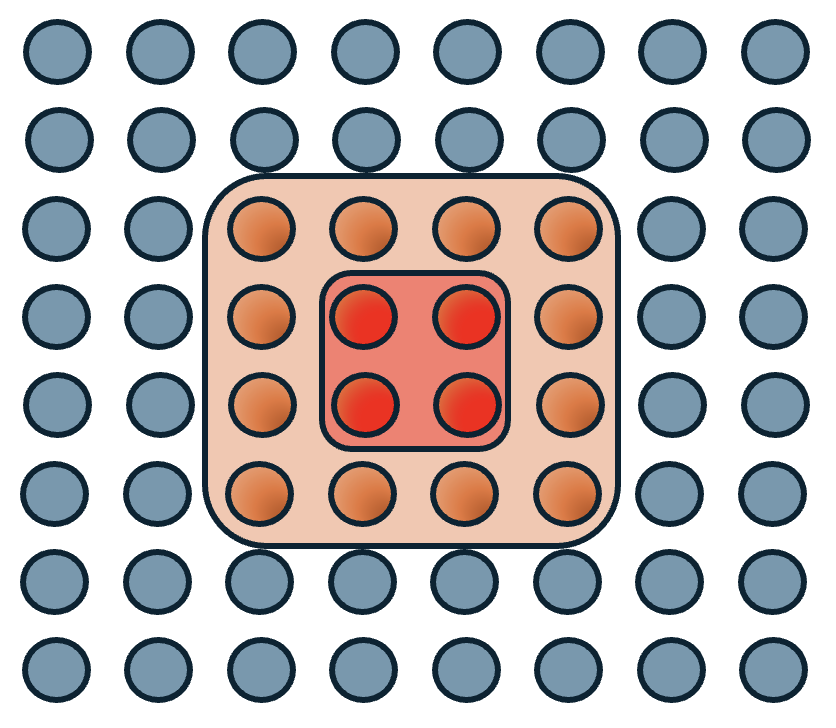
\includegraphics[width=0.5\textwidth]{Images/Bain.png}
    \caption{Schematic representation of the three region composing the embedding. red: cluster, orange: TIPS, blue: point charges}
    \label{Bain}
\end{figure}
Another problem in selecting fragments in ionic crystal is the overall charge of the fragment.
The centre of the study is the metallic ions, charged positively, forming ionic bonds with negatively charged ligand.
A correct description of these magnetic centre requires to include all closest neighbors which makes the overall fragment negatively charged.
The ions at the border of the fragment, replaced by point charges, are then positive. This induces a polarization of the electron density of the anions bordering the cluster.
To avoid the electrons escaping the fragment, pseudo-potentials are placed at the lattice sites near the fragment to act as walls which prevent electrons from approaching these positive charges as if they were real atoms.

Two procedure were explored to create such embedding:
\begin{itemize}
    \item[(1)] Formal charges were used in a sphere with very large $R_c$ (around 50 \AA{}).
    \item[(2)] Optimised point charges were obtained using Ewal Summation from formal charges, this allows to reduce the $R_c$ to a few angstrom around the fragment.
\end{itemize}

These potentials are called Total-Ion-Potentials (TIPS) and can be either \textit{ab} \textit{initio} model potential (AIMP) or Effective Core Potential (ECP) depending on which Quantum Chemistry software is used.
All of this is done to ensure that the properties extracted from the fragment, \textit{i.e} a finite system, are a good representation of the crystal properties, \textit{i.e} an infinite system.

\subsection{Effective Hamiltonian}

Having ways to compute the \textit{ab} \textit{initio} multi reference wave functions usually leads to lenghty expression where the wave function is spanned along a large number of Slater determinant making its analysis complicated.
On the other hand, the model Hamiltonian work in a much smaller space where a small number of electrons is used to introduce effective interactions.
A way to connect the two Hamiltonians is to apply a theory developped by Bloch called Effective Hamiltonian theory. 
Its purpose is to build an effective Hamiltonian whose eigenvalues reproduce the energy spectrum of the \textit{ab} \textit{initio} Hamiltonian but using a much smaller number of eigenfunctions.



Starting from the Schrodinger equation with the Born-Oppenheimer Hamiltonian $\hat{H}$:

\begin{equation}
    \hat{H}\ket{\Psi_m}=E_m\ket{\Psi_m}
\end{equation}

Where $\Psi_m$ are the eigenvectors with the associated eigenvalue $E_m$ forming the space $S$ of size $N$. 
We define a smaller space $S_0$ with $N_0$ states, this space is usually composed of the low lying state where the model Hamiltonian will be developped.
An effective Hamiltonian $H_{eff}$  is built to reproduce the energy spectrum of the exact Hamiltonian in the target space $S_T$ using a small number of low-lying states $\tilde{\Psi}_m$ such that:

\begin{equation}
    \hat{H}_{eff}\ket{\tilde{\Psi}_m}=E_m \ket{\tilde{\Psi}_m}
\end{equation}
This target space $S_T$ is chosen to be the same as the model space $S_0$ allowing for direct comparison.
The first step is to project the eigenfunctions $\Psi_m$ onto the model space using the projector:

\begin{align}
    \hat{P}_0=\sum_{m}^{N_0} \ket{\tilde{\Psi}_m} \bra{\tilde{\Psi}_m}\\
    \ket{\tilde{\Psi}_m}=\hat{P}_0 \ket{\Psi_m}
\end{align}

These eigenvectors are not necesserily orthogonal leading to a non-Hermitian Hamiltonian, this is problematic when comparing to the model Hamiltonians which are Hermitians.
In this work, we apply the formalism proposed by Des Cloizeaux where the vectors are symmetrically orthonalized from the overlap matrix $S$:

\begin{equation}
    \ket{\tilde{\Psi}_m^\bot}=S^{-1/2} \ket{\tilde{\Psi}_m}
\end{equation}

At this point, it is possible to check the quality of the target space by calculating the norm of the projected vectors.
If too small, the interactions of the system are not captured correctely by the model space making it inadecate. 
\par When these projections are close to one, we can consider the model space adecate, the effective Hamiltonian is then built:

\begin{equation}
    H_{eff}=\sum_{m}^{N}\ket{\tilde{\Psi}_m^{\bot}}E_m \bra{\tilde{\Psi}_m^{\bot}}
\end{equation}

Once this is done, this numerical matrix $H_{eff}$ constructed from the $\textit{ab}$ $\textit{initio}$ exact Hamiltonian are compared to the model Hamiltonian representation matrix. 
This allows for the extraction of values for the model Hamiltonian parameters as well as a test of validity.
If there is too much deviation between the two matrices, it is possible that there is some missing interaction in the model.

\chapter{Study of the anisotropy in mononuclear complexes}

The field of mononuclear complexes is a perfect area for the study of magnetic anisotropy. 
The finite size of such complex as well as the localised character of the interaction allow for the explicit treatment of all atoms at play with reasonnable computational cost.
This combined with the large amount of experimental data available allow for the validation of models and computational methodology.
Numerous studies were dedicated to the application of the ZFS model Hamiltonian on mononuclear complexes based on fourth period transition metal.
It has established that the value of the ZFS parameters are highly dependant on the metallic ion and its environment, the choice of ligand is crucial as we will see in this chapter.
\par State of the art methodology for such study is to generate a wavefunction from a CASSCF calcuation including all electronic state generated by an active space composed of all the d orbitals of the metallic ion and the electrons occupying them. 
Dynamic correlation is taken into account by pertubation with NEVPT2 including all the states from the CASSCF calculation. 
Spin orbit coupling between $M_S$ component of all states are accounted for using Spin-Orbit-State-Interaction with NEVPT2 correlated energies as the diagonal of the SO matrix.
Finally, ZFS parameters are extracted following the Effective Hamiltonian Theory in a procedure implemented in the ORCA package.

\section{First Order Spin Orbit Coupling}

The ideal case for creating large anisotropy is to approach first order spin orbit coupling regime. 
First order spin orbit coupling arises when a two-fold degenerate ground state is formed from configuration with degenerate d-orbitals as represented on figure \ref{Fer_config} in case of $d^6$ configuration in $D_{5h}$ geometry.

\begin{figure}[h!]
    \centering
    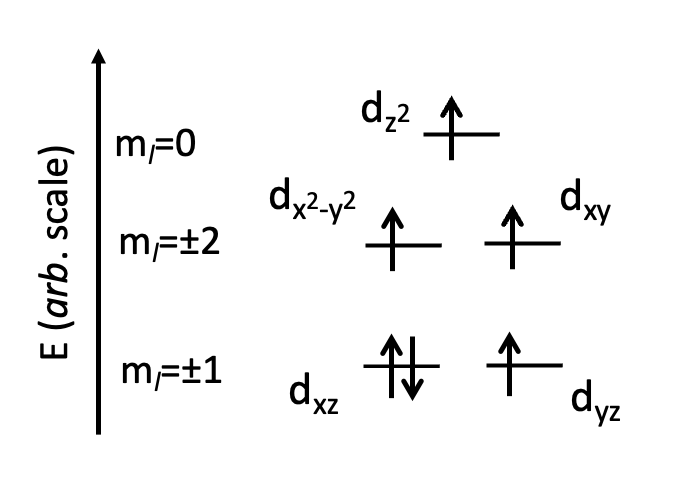
\includegraphics[width=0.5\textwidth]{Images/DiagOrbFed6.png}
    \caption{The two degenerate configurations for $d^6$ configuration in ideal $D_{5h}$ geometry}
    \label{Fer_config}
\end{figure}

These two states would be strongly coupled via 1$^{st}$order SOC resulting in a large splitting of the $M_S$ component of the ground state with a large value for the D term as strong as the spin orbit coupling constant.
In reality a lift of degeneracy of the d orbitals is induced from the coordination sphere stabilising one of the two configurations, making it the main component of the ground state, and destabilising the other to an excited state.
This loss of symmetry greatly reduces energy splitting of $M_S$ component and may induce rhombicity in the system. 
At this stage the angular momentum L is quenched making the spin momentum S a "not-too-bad" quantum number, allowing the application of the ZFS model Hamiltonian formalism with the extraction of a $D$ axial parameter and rhombic terme $E$.
The remaining anisotropy is the result of second order spin orbit coupling from the ground state with low-lying exicted states.
This interaction stems from the excitation of an electron from a d orbital to a higher-energy orbital as depicted on figure \ref{excitattionanisotropie} and its magnitude rely on the difference in energy between the orbitals.
Small energy differences (a few hundred cm$^{-1}$) between the orbital allow to retrieve a contribution of 1$^{st}$order SOC increasing the value of D.
It has then become an interest to find ligands that satisfy this condition of quasi-degeneracy of the d-orbital.

With this in mind, a series of five Iron(II) complexes were synthesized in a heptacoordinated environment with different apical ligands (X and Y position in figure \ref{FeComplex}).
\begin{figure}[h!]
    \centering
    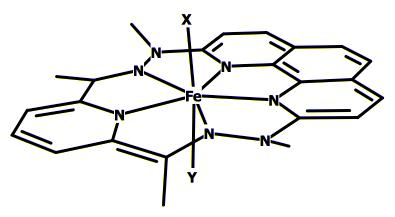
\includegraphics[width=0.5\textwidth]{Images/ComplexFe.XY.jpg}
    \caption{Schematic representation of the complex with H atoms attached to carbon hidden}
    \label{FeComplex}
\end{figure}



\section{Impact of the Electric field on the ZFS parameters}

This chapter is the follow up of a previous study on a Nickel II complex exhibiting large unaxial anisotropy.
This complex is formed from a tetradant ligand (hexathyl-2,2',2''-triamino-triethylamine) with three Nitrogens forming in plane bonds with the metal ion, the fourth Nitrogen forms a bond in the perpendicular plane as shown on figure \ref{NiMe6tren}.
At the opposite of this fourth Nitrogen a halide apical ligand is found, Chlorine or Bromine.

\begin{figure}[h!]
    \centering
    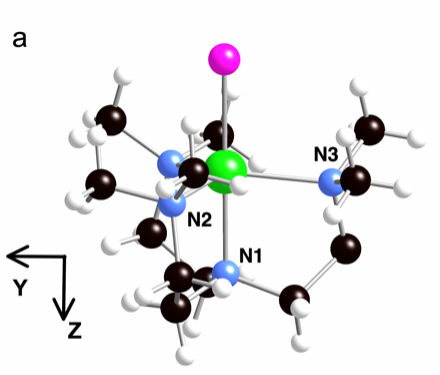
\includegraphics{Images/NiMe6trenTalal.png}
    \caption{Representation of the complex [Ni(Me6trenCl)](ClO4), Ni in green, Cl, N in blue, C in black and H in white}
    \label{NiMe6tren}
\end{figure}

Cristallographic data indicates that this complex crystallises in the trigonal space $R3c$ with a $C_3$ axis of symmetry along the Ni-Cl axis.
This coordination induces a degeneracy of the d-orbital which share the same angular component $m_l$, \textit{i.e} $d_{xy}$($d{xz}$) and $d_{x^2-y^2}$($d_{yz}$). 
Conditions for 1$^{st}$ order SOC are met between two degenerate ground state carried by the two $d^8$ configurations depicted on figure \ref{NiMe6tren_config}
This would result in a large splitting of the $M_S$ component of the ground state with a large value for the D term as strong as the spin orbit coupling constant of the nickel ion ($\xi_{Ni}$=644cm$^{-1}$).
At this stage, a competiting effect appears, the Jahn-Teller effect which break the orbital degeneracy by deforming the ligand which in turn reduces the axial anisotropy and give rise to non-zero rhombic term (E$\neq$0).
This distortion is confirmed by both eletron paramagnetic resonance (EPR) studies and theoretical study, this revokes the possibility of 1$^{st}$order SOC leaving only 2$^{nd}$order SOC at the origin of the anisotropy.

\begin{figure}
    \centering
    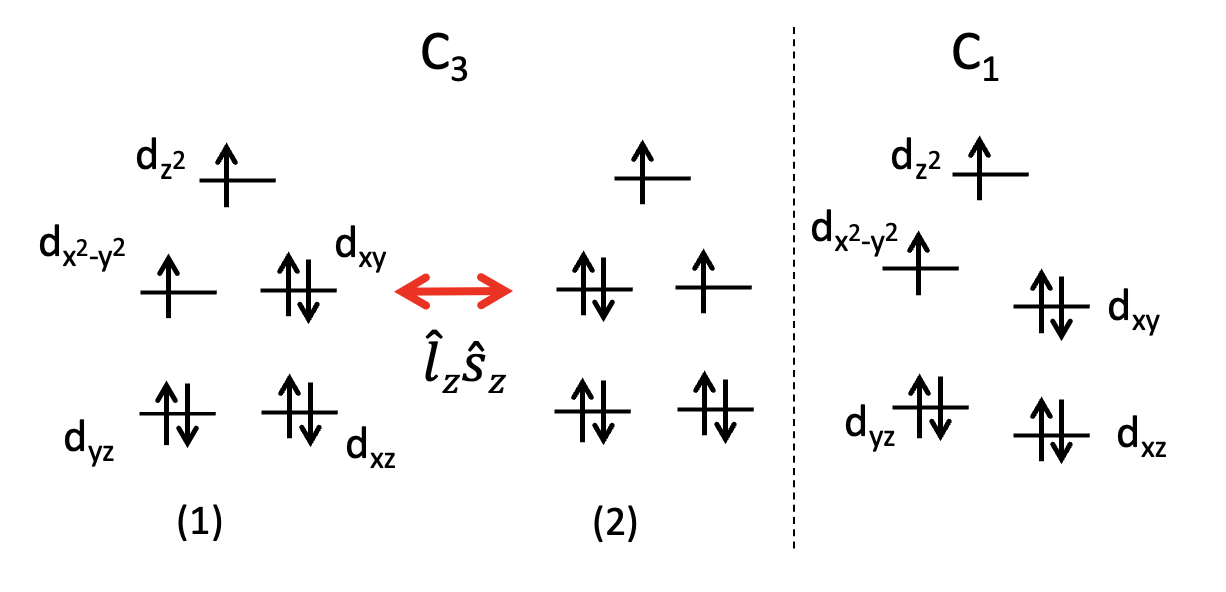
\includegraphics[width=0.5\textwidth]{Images/NiMe6tren_config.png}
    \caption{Energy diagrams of the d orbitals in case of three-fold symmetry $C_3$ (left) and in presence of Jahn-Teller distortion (right) with the induced lift of degeneracy of the d-orbitals. }
    \label{NiMe6tren_config}
\end{figure}

The ground state is now mainly carried by the configuration shown on figure \ref{NiMe6tren_config} where the $d_{x^2-y^2}$ is simply occupied while the $d_{xy}$ stays doubly occupied.
The concluding remark of this study was that this complex shows a large axial anisotropy with $D\approx-120cm^{-1}$ and a significant rhombic term $E$=1.6cm$^{-1}$. 
While the Jahn-Teller effect has a large impact on the values of the D paramter, it is not able to completely negate it showing that the ligand rigidity is on par with the distortion.

\par The focus of our study lies in the interest of controlling the anisotropy via an external stimulus such as an electric field.
Indeed, while the effect of magnetic field on the different $M_S$ component is well known with the Zeeman Effect, it is practically impossible to focus a magnetic field at the nanoscale.
This is not the case for electric field which allows very accurate control at this scale and can affect the magnetic properties of a material via Magneto-Electric couplings.
\textit{Ab} \textit{initio} calculations allow for the appreciation of the Jahn-Teller distortion as well a the determination of the anisotropic parameters D and E as a function of the applied electric field.
The rationalization of such mechanism comes from the analysis of the spin-orbit coupled wave-function and the contribution of the excited states to the ZFS both provided by the ORCA program.
The  origin of this Magneto-Electric effect is believed to come from both electronic and geometric structure changes under the applied electric field. 
To identify and quantify these mechanisms, the electric field was applied under two different orientations in three types of calculations:

\begin{itemize}
    \item[(a)] eletronic structure changes, ZFS calculation under an applied field on the zero-field geometry
    \item[(b)] geometric structure changes, ZFS calculation under no applied field on the field-optimised geometry.
    \item[(c)] combined eletronic and geometric, both geometry optimisation and ZFS calculation performed under an applied electric field
\end{itemize}

To explore the different response to the electric field given its orientation, the field F was first applied along the Ni-Cl axis that corresponds to the easy axis of magnetization.
This orientation include the maximal component of the dipole moment and will be referred as F//Z.
It was then applied in a perpendicular direction (F//Y) in the YZ plane that include the Ni, N1 and N3 atom (refer to figure \ref{NiMe6tren} for numerotation of atoms). 
This axis was chosen as the Ni-N3 bond length is the shortest among the three Ni-N bonds in the XY plane.

\subsubsection*{Analysis of the contribution}

The main contribution to the D term comes from the SOC with the first excited triplet state ($T^1$) which is mainly expressed on the determinant created by exciting an electron occupying the $d_{x^2-y^2}$ to the $d_{xy}$.
The Hamiltonian used to rationalize the SOC is given by $\hat{H}^{SO}=\sum_{i} \zeta(\hat{l}_x^i\hat{s}_x^i+\hat{l}_y^i\hat{s}_y^i+\hat{l}_z^i\hat{s}_z^i)$ where $i$ runs over all the electrons of the $d^8$ configuration.
The two lowest triplet are formed primarily from orbitals that are combination of $m_l$=$\pm$2, the resulting SOC then originate only from the $\hat{l}_z^i\hat{s}_z^i$ part of the Hamiltonian between the $m_s$=$\pm$1 of each triplet.
This coupling tends to stabilise the $m_s$=$\pm$1 of the $T_0$ ground state without affecting the $m_s$=0 component, which gives a negative contribution to the D term.
This contribution can be estimated at second order perturbation:
\begin{equation}
    C(D)^{(2)}=-\frac{|\bra{T^0_{\pm1}}\hat{H}^SO\ket{T^1_{\pm1}}|^2}{\Delta E}
\end{equation}
With $\Delta E = E(T^1)-E(T^0)$ being the energy difference between the two states.
As the difference in energy is relatively small, a better treatment of this contribution can be obtained variationally by diagonalizing the 2$\cross$2 SOC matrices in the basis of $T^0_{\pm1}$ and $T^1_{\pm1}$:
\begin{equation}
    C(D)_{VAR}=\frac{\Delta E -\sqrt{\Delta E^2+4|SOC|^2}}{2}
\end{equation}
Where $|SOC|^2$ is the square value of the off-diagonal term in $\hat{H}^{SO}$ between ground and excited components.
Other states may contribute positively or negatively to the overvalue value of D, their contribution can be obtained the same way. 
However the variation of the electric field has almost no impact on those other contributions, as such they will be left out of the rationalization.


\chapter{Electric field on Exchange anisotropy}\label{chap:Cu2Cl5}

This study is part of a series of work that aims to rationalize the origin of exchange anisotropy in polynuclear molecules.
In order to achieve this, a procedure of extraction was developped to obtain the parameter present in the Multi-Spin Hamiltonian, namely the Dzyaloshinskii-Moriya pseudo-vector $\vb{d}_{AB}$ and symmetric tensor of exchange $\overline{\overline{D}}_{AB}$:

\begin{equation}
        \hat{H}_{AB}=J(\hat{\vb S}_A \cdot \hat{\vb S}_B) + \hat{\vb S}_A \cdot\overline{\overline{D}}_{AB} \cdot \hat{\vb S}_B + \vb{d}_{AB} \cdot (\hat{\vb S}_A \cross \hat{\vb S}_B)
\end{equation}

This procedure was tested on a simple model molecule composed of two $Cu{2+}$ ion with $Cl^-$ ions as ligands as represented on figure \ref{MolCu2Cl5}. 
This system was chosen because of its simplicity, with only one magnetic electron per center and a reasonnable size it allows for simple analytical derivation and high level treatment of the correlation.
Such a toy molecule can also be modeled to assess the impact of geometry, \textit{i.e} distances and angles, on these interactions.
It was first determined how to create giant Dzyaloshinskii-Moriya interaction by modifying the $\theta$ angle.

\chapter{Herbertsmithite}

introduction sur les liquides de spin

\subsubsection*{Computational Informations}

The structure studied was taken from a X-ray study, the Hydrogen position were optimised using periodic DFT with PBE functional on the Quantum Espresso code.

Density functional theory calculations were performed on the ORCA package with def2-TZVP basis set on all atoms and the $\omega$B97X-D3 functional which has shown to provide very good value of magnetic couplings.
Wave-function base method were carried out on the MOLCAS program and CASDI codes with the extendend ANO-RCC basis set (6s5p3d2f for Cu and Zn, 4s3p2d
for O, 4s3p1d for Cl and 2s1p for H)

The embedding's pseudopotential were set to the SDD Effective Core Potentiel (ECP) for ORCA calculations and \textit{ab} \textit{initio} model potentials (AIMP) of MOLCAS calculations. 
The quality of the embedding was checked by comparing the value of $J_1$ using the B3LYP functional for embedded cluster and periodic calculations (using the Crystal code). 
The J1 values are in perfect agreement: 240K for periodic and 239K for embedded cluster. 
As we will see below, these B3LYP values slightly overestimate the coupling but demonstrate the adequacy of the material model adopted in this study.

\subsection{DFT study}

In a first approximation, the isotropic behavior of Herbertsmithite is described by an unique first neighbor coupling. 
The highly-correlated nature of such system suggests the possibility of longer range interaction between copper ions by one or more neighbor. 
To explore this possibility, the need to compute large fragments arises making the appplication of wave-function based method complicated.
First the number of Cu$^{2+}$ into the fragment has a direct impact on the size of the active space, even restricting to one orbital/ one electron per copper centrer lead to convergence trouble in the calculation.
Also, the number of determinant and spin states generated forbid the use of Post-CASSCF method which are crucial for good estimation of magnetic couplings.
Finally, the number of spin states render the analytical derivation complicated with large matrices to diagonalize.
As such, Density Functional Theory provides a good middle ground to compute large systems. 
It also presents some incoveniences, the DFT wavefunction is monodeterminantal and usually not an eigenfunction of the $\hat{S}^2$ operator which prevents the use of the HDVV Hamiltonian.
Nevertheless, the combinated use of Broken-Symmetry DFT (BS-DFT) and the Ising Hamiltonian provides a good way to obtain an estimation of the couplings in the system.
The Broken-Symmetry approach rely on the computation of DFT solutions where the $M_S$ value of spin moment of each copper ion of the fragment have been imposed beforehand to $\pm \frac{1}{2}$. 
It is then possible to obtains multiple solutions per fragments to make a connection between the energy differences of each solutions and the Ising Hamiltonian.
Additionaly, the time necessary for a DFT calculation and for the derivation of its analytical solution allows for the exploration of different properties of the embedding such as the size of the fragments and overall quality of it.


\subsubsection*{In-plane couplings}

In a first description, a fragment presenting only the first neighbor coupling was introduced with three copper ions as shown on figure \ref{FragmentDFT}.
Four solutions are possible to compute with $M_S$$\ge$$0$, first a $M_S=3/2$ where all magnetic moment of the Cu$^{2+}$ ions are aligned creating a fully ferromagnetic solution. 
Then three other solutions are possible by switching the $M_S$ value of one of the Cu$^{2+}$ ion to $-1/2$. 
If the choice of fragment and construction of the embedding are done correctely, this should lead to three equal differences of energy as these solutions are treated equally by the Ising Hamiltonian.

\begin{figure}[h!]
    \centering
    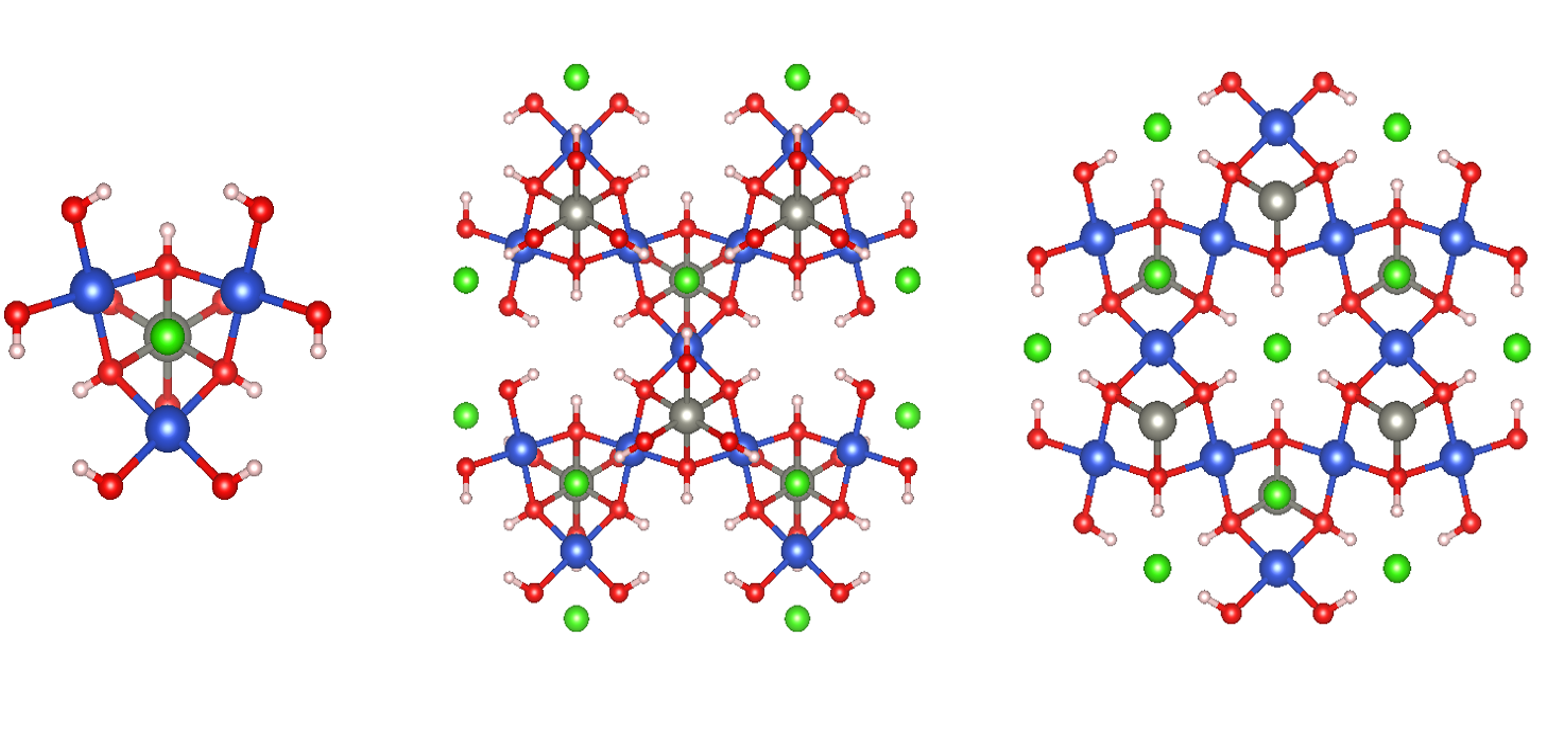
\includegraphics[width=0.8\textwidth]{Images/FragmentDFT_plan.png}
    \caption{Fragments considred for DFT calculations for in plane component, (a) trimer (b) 13Cu (c)12Cu}
    \label{FragmentDFT}
\end{figure}

Let us call the highest occupied orbital of each copper ion a,b and c. 
The Slater determinant describing the high spin solution ($M_S$=$+1/2$ on each Cu$^{2+}$) can then be written $|abc|$ while the low spin solutions (one of the $M_S$ value is switched to $-1/2$) are written $|ab\overline{c}|$,$|a\overline{b}c|$ and $|\overline{a}bc|$.
Applying $\hat{H}_{Ising}=\sum_{i,j}J_1 \hat{S}_{i,z}\hat{S}_{j,z}$ to the high spin (HS) solution $|abc|$ gives the eigenvalue $\frac{3}{2}J_1$ while the application on the low spin (LS) solutions gives the eigenvalue $\frac{1}{2}J_1$. 
The Ising Hamiltonian has no effect on the spin variable of each centre, hence its matrix representation is diagonal:

\begin{center}
    \begin{tabular}{c | c c c c}
        $H_{Ising}$ &$|ab\overline{c}|$&$|a\overline{b}c|$ & $|\overline{a}bc|$\\
        \hline
        $|abc|$ & $\frac{3}{2}J_1$ & 0 & 0 & 0\\
        $|ab\overline{c}|$ & 0 & $\frac{1}{2}J_1 $& 0 & 0\\
        $|a\overline{b}c|$ & 0 & 0 & $\frac{1}{2}J_1 $ & 0 \\
        $|\overline{a}bc|$ & 0 & 0 & 0 & $\frac{1}{2}J_1 $
    \end{tabular}
\end{center}

The value of $J_1$ can then be extracted from the difference in energy between the high spin solution and low spin one:
\begin{equation}
    J_1=E_{HS}-E_{LS}
\end{equation}

The same procedure of extraction can now be applied to larger fragment with the introduction of longer range couplings.
The second fragment created included nice copper ions in total which allowed for the consideration of two new coupling, $J_2$ and $J_3$ represented on figure \ref{CouplageDFT}.
It indicated that these couplings were small ($|J_{2}|\approx |J_{3}|\approx1 cm^{-1}$ each) with a large standard deviation.
While these results provided good hindsight on the nature of these two couplings, the extraction was unsatisfactory.
The source of this deviation is believed to be the environment of ions taking part in the interaction. 
These couplings involve ions at the border of the fragment whose neighboring atoms were not always explicitely computed compared to ions at the center of the fragment.
As such, small convergence differences could alter the energy value obtained via DFT and cause such small deviation, for .
It was decided to increase the size of the fragment to twelve and thirteen copper ions (fragment (c) and (b) from figure \ref{FragmentDFT}) so that there would be ways account for these interaction within the center of the fragment.


\begin{figure}[h!]
    \centering
    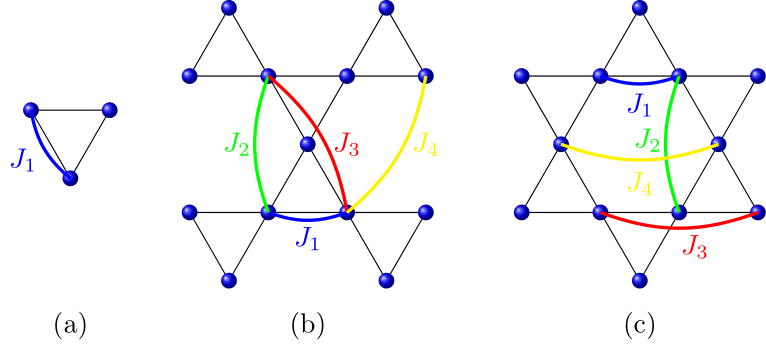
\includegraphics[width=0.8\textwidth]{Images/ModeleDFT_plan.png}
    \caption{Schematic representation of the fragments and the couplings introduced}
    \label{CouplageDFT}
\end{figure}

The results obtained for each couplings in the thre fragments are presented in table \ref{ResultatsDFT}.
The first thing to note is the good transferability with a small relative deviation from one cluster to the other.
Note that with this convention of the Ising Hamiltonian (a plus sign in front of the $J$ term), a positive value indicates antiferromagnetism while negative indicates ferromagnetism.
The closest neighbor interaction $J_1$ is in good agreement with values published in the litterature while $J_2$,$J_3$ and $J_4$ are very weak. 

\begin{center}\label{ResultatsDFT}
    \begin{tabular}{c c c c c}
        \hline
        $J_i (K)$ & (a) & (b) & (c) & $d_{Cu-Cu}$ (\AA{}) \\
        \hline
        $J_1$ & 178.0 & 191.2 & 181.0 &3.42\\
        $J_2$ & - & 0.5  & 0.4& 5.91\\
        $J_3$ & -& -1.1& -1.0&6.83\\
        $J_4$ & -& -0.1 & -0.2& 6.83\\
        \hline
    \end{tabular}
\end{center}

These results highlight the mainly antiferromagnetic nature of these interactions with a leading interaction $J_1$ at least two order of magnitude higher than the other.
This confirm the the use of models composed of only one $J$ interaction, the negligenge of other couplings should cause no more than a small deviation.

\subsubsection*{Out-of-plane coupling}

Another preoccupation of the model is the occupation disorder, cristallographic studies have identified two types of defects present at low-temperature. 
First the substitution of the $Zn^{2+}$ inter-plane site with a $Cu^{2+}$ ion, estimated with a 0.15 occurance rate, and second an $Zn^{2+}$ entering the Kagome plane with a much smaller occurance rate (<0.05).
In a similar approach, three clusters that were built to include the intersite ion are represented on figure \ref{fig:FragmentIntersite}.
Fragment (a) was designed to check the $J_1$ coupling, fragment (b) and (c) allow the exploration of both type of disorder.

%\begin{figure}[h!]
%    \centering
%    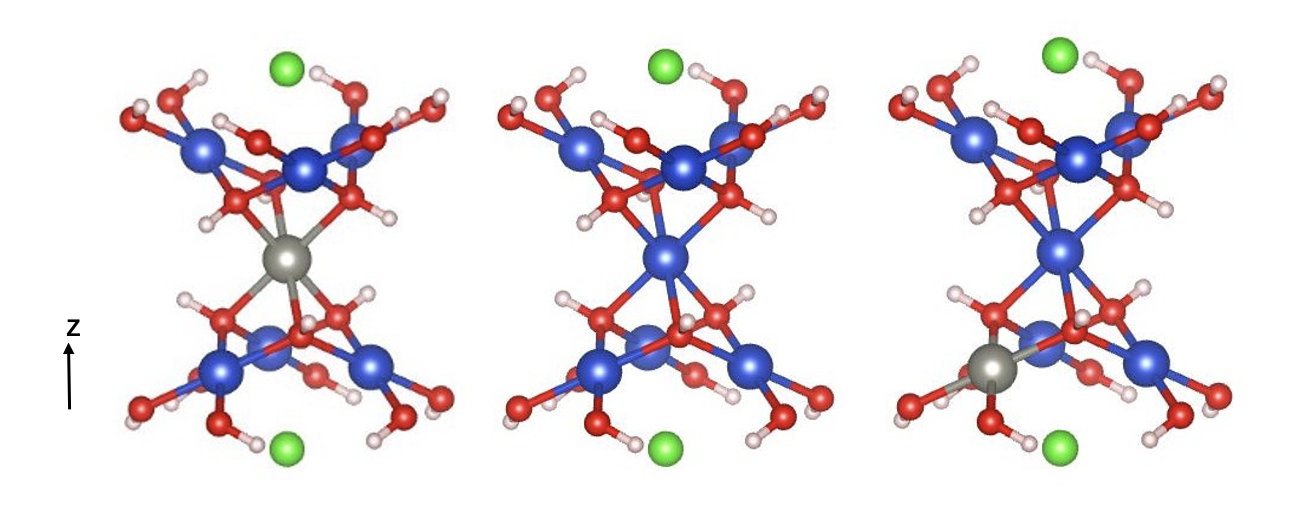
\includegraphics[width=0.8\textwidth]{Images/FragmentDefauts.png}
%    \caption{Fragments considred for DFT calculations for in plane component, (a) trimer (b) 13Cu (c)12Cu}
%    \label{FragmentIntersite}
%\end{figure}

\begin{figure}[!h]
    \centering
    \begin{subfigure}{.5\textwidth}
      \centering
      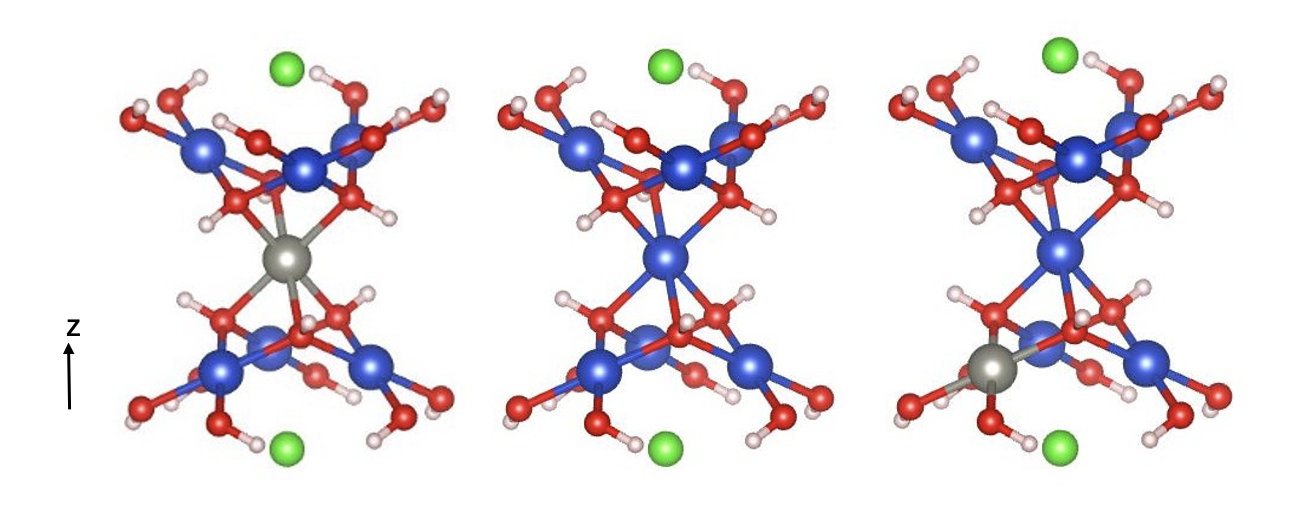
\includegraphics[width=\linewidth]{Images/FragmentDefauts.png}
      \caption{\textit{ab} \textit{initio}}
      \label{fig:FragmentIntersite}
    \end{subfigure}%
    \begin{subfigure}{.5\textwidth}
      \centering
      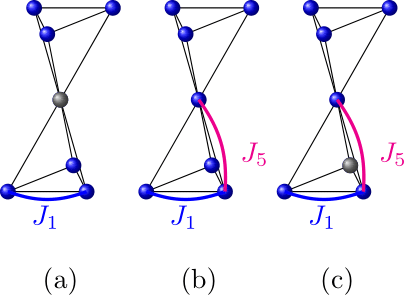
\includegraphics[width=\linewidth]{Images/ModeleDFT_interplan.png}
      \caption{Couplings}
      \label{fig:CouplingsInterplan}
    \end{subfigure}
    \caption{Embedded clusters and associated model for intersite calculations}
    \label{fig:FragmentInterplan}
    \end{figure}

These fragments allows for the introduction of a new coupling $J_5$ between the intersite $Cu^{2+}$ ion with an inplane one.
Note that with a distance $d_{Cu-Cu}=3.07$\AA, it actually becomes the first neighbor coupling.
Table \ref{ResultatsIntersite} shows a $J_1$ coupling in accordance with previous calculation in all three clusters with now the presence of strong ferromagnetic coupling $J_5$.
Its magnitude, $J_5\approx - J_1/2$, could have a strong impact on the properties of this material and should in fact be taken into account in the model.
Due to this magnetic coupling, Herbertsmithtie might not be the perfect realisation of a Kagome-antiferromagnet and explain the difficulty to determine its nature as spin liquid.

\begin{center}\label{ResultatsIntersite}
    \begin{tabular}{c c c c }
        \hline
        $J_i (K)$ & (a) & (b) & (c)  \\
        \hline
        $J_1$ & 184.2 & 184.1 & 182.7 \\
        $J_5$ & - & -83.4  & -82.0\\
        \hline
    \end{tabular}
\end{center}


\subsection{Wave-Function Theory study}

A second purpose of this study was the determination of anisotropic interaction in the crystal.
The extraction of such interactions follows the same procedure as described in chapter \autoref{chap:Cu2Cl5}.
The computation of SO-states being very computationally demanding, this extraction will be resticted to two fragments of small size.


\begin{figure}
    \centering
    \begin{subfigure}{.5\textwidth}
      \centering
      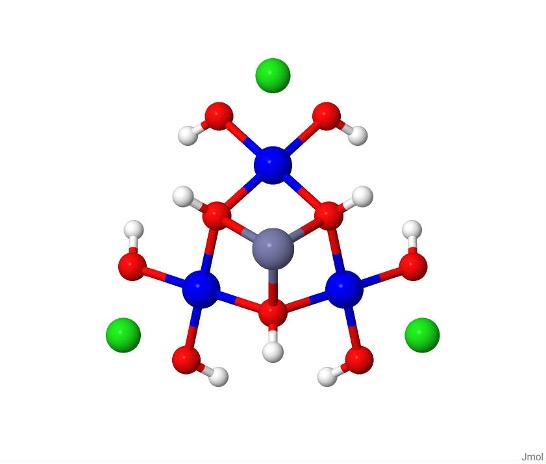
\includegraphics[width=\linewidth]{Images/Trimere.jpg}
      \caption{Trimer}
      \label{fig:subtrimer}
    \end{subfigure}%
    \begin{subfigure}{.5\textwidth}
      \centering
      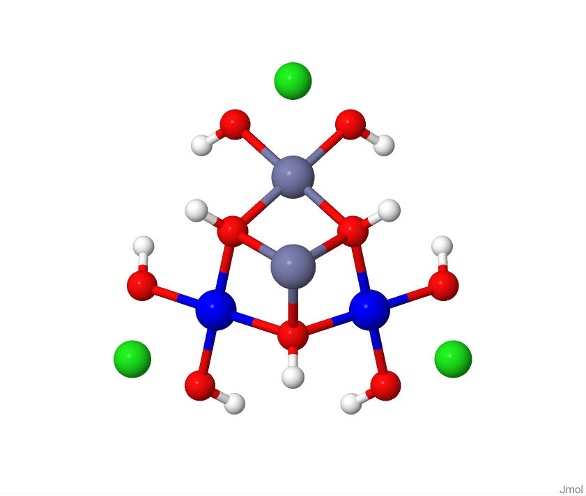
\includegraphics[width=\linewidth]{Images/Dimer.jpg}
      \caption{Dimer}
      \label{fig:subdimer}
    \end{subfigure}
    \caption{Embedded clusters used for Wave-funciton computation}
    \label{fig:FragmentWF}
    \end{figure}

The first fragment, figure \ref{fig:subtrimer}, is similar to the one used for DFT calculation, with three copper ions arranged in an equilateral triangle. 
A second fragment was designed by substituting one of the $Cu^{2+}$ with a diamagnetic $Zn^{2+}$.
As the d shell of the zinc ion is completely filled it will not take part in the magnetic interactions, leaving us with essentially a dimer which capture the interaction of only two $Cu^{2+}$.

\subsubsection*{Isotropic Coupling}

To check the applicability of WFT calculation to this system, the first step was to try and reproduce the value of $J_1$.
In both cluster, two type of active space were considered:
\begin{itemize}
    \item one electron and orbital per magnetic center
    \item all eletronc occupying the d shell of each magnetic center
\end{itemize}

The first type of active space results in a CAS(2,2) for the dimer calculation which generates one triplet (S=1) and one singlet (S=0) state.
\begin{align}
    &\ket{1,1}=|ab|\\
    &\ket{1,0}=\frac{1}{\sqrt{2}}(|a\overline{b}|-|b\overline{a}|)\\
    &\ket{1,-1}=|\overline{a}\overline{b}|\\
    &\ket{0,0}=\frac{1}{\sqrt{2}}(|a\overline{b}|+|b\overline{a}|)
\end{align}

The value of $J_1$ is then given by the difference in energy between the triplet and singlet state $J_1=E(S=1)-E(S=0)$.
The enlarged active space CAS(18,10) generates 25 Triplet and 25 Singlet states.

In the case of the trimer cluster, CAS(3,3) represents the minimum active space which generates 1 quartet (S=3/2) state and two doublet (S=1/2) states. The two doublet are degenerate if only one value of $J$ is taken into account as is our case with an equilateral repartition of the copper ions.
\begin{align}
    &\ket{3/2,3/2}=|abc|\\
    &\ket{3/2,1/2}=\frac{1}{\sqrt{3}}(|ab\overline{c}|+|a\overline{b}c|+|\overline{a}bc|)\\
    &\ket{1/2,1/2}_1=\frac{1}{\sqrt{6}}(|ab\overline{c}|+|a\overline{b}c|-2|\overline{a}bc|)\\
    &\ket{1/2,1/2}_2=\frac{1}{\sqrt{2}}(|ab\overline{c}|-|a\overline{b}c|)
\end{align}
The expression of the $m_s$ component with negative value were left out as they only differ by the number of up and down spins.
The value of $J_1$ is then given by $J_1=\frac{2}{3}(E(S=3/2)-E(S=1/2))$.
The enlarges active space CAS(27,15) generates 125 Quartet and 250 Doublets states.

CASSCF calculation tends to "over"-localise the wavefunction on the metallic center, thus underestimating mechanism at the origing of the antiferromagnetic contribution to the $J$ integral.
As such it does not provides a good estimate but can nevertheless give information about the nature of the coupling.
Table \ref{ResultatsWFT} shows the results obtained at multiple level of calculation for different active space.

\begin{center}\label{ResultatsIntersite}
    \begin{tabular}{c c c c c c }
        \hline
        $J_1 (K)$ & CAS(2,2)/CAS(3,3) & CAS(18,10)/CAS(27,15) & CASPT2 & DDCI1  & DDCI3  \\
        \hline
        Dimer & 10.7 & 8.3 & 69.8 & 50.0 & 80.1 \\
        Trimer & 8.2 & 7.7 & 56.0  & 50.7 & 60 \\
        \hline
    \end{tabular}
\end{center}





\end{document}
